\documentclass[11pt, oneside]{article}   	% use "amsart" instead of "article" for AMSLaTeX format
\usepackage{geometry}                		% See geometry.pdf to learn the layout options. There are lots.
\geometry{letterpaper}                   		% ... or a4paper or a5paper or ... 
%\geometry{landscape}                		% Activate for for rotated page geometry
%\usepackage[parfill]{parskip}    		% Activate to begin paragraphs with an empty line rather than an indent
\usepackage{graphicx}				% Use pdf, png, jpg, or eps� with pdflatex; use eps in DVI mode
								% TeX will automatically convert eps --> pdf in pdflatex		
\usepackage{amssymb}
\usepackage{amsmath}
\usepackage{parskip}


\title{Limit Problems}
%\author{The Author}
%\section{}
% \subsection*{R code}
\date{}							% Activate to display a given date or no date

\graphicspath{{/Users/telliott_admin/Dropbox/Tex/png/}}
% \begin{center} 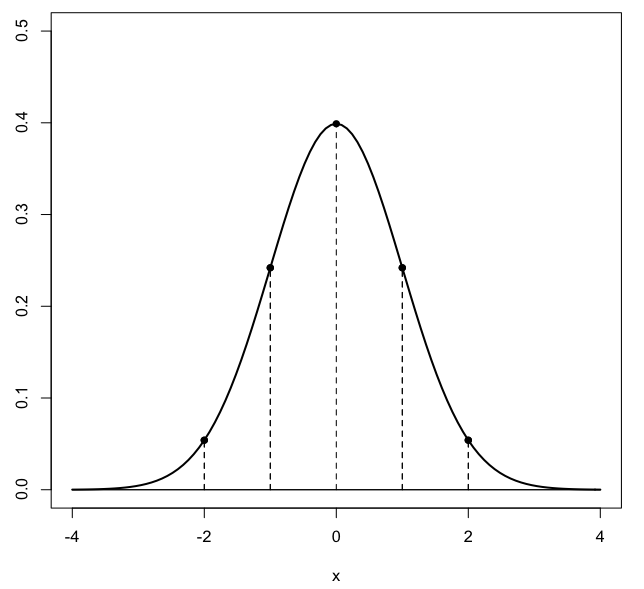
\includegraphics [scale=0.4] {gauss3.png} \end{center}

\begin{document}
\maketitle
\large

\subsection*{Factoring}
Factoring is OK when evaluating a limit.  For example
\[ \lim_{x \rightarrow 2} \ \frac{x^2 + 4x - 12}{\ x^2-2x} \]
Plugging in $x=2$ gives $0/0$.  We notice we can factor the numerator and the denominator
\[ = \lim_{x \rightarrow 2} \ \frac{(x+6)(x-2)}{\ x(x-2)} \]
Now, since we are \emph{not interested} in what happens at $x=2$, we can cancel here, giving
\[ = \lim_{x \rightarrow 2} \ \frac{(x+6)}{x} = \frac{8}{2} = 4 \]

\subsection*{Conjugate}
\[ \lim_{x \rightarrow 4} \ \frac{\sqrt{x} - 2}{\ x-4} \]
Substitution gives $0/0$.  We try multiplication by the conjugate
\[ \frac{\sqrt{x} - 2}{\ x-4} = \frac{\sqrt{x} - 2}{\ x-4} \ \frac{\sqrt{x} + 2}{\sqrt{x} + 2} \]
The numerator gives $x-4$, and  before you rush to do the denominator, notice the cancellation:
\[ = \frac{x - 4}{(x-4)(\sqrt{x} + 2)} \]
So this is just
\[ \lim_{x \rightarrow 4} \  \frac{1}{\sqrt{x} + 2} = \frac{1}{4}  \]

\subsection*{Polynomial as $x \rightarrow \infty$}
\[ \lim_{x \rightarrow \infty} \ 3x^2 + 2x + 1 \]
\[ = \lim_{x \rightarrow \infty} \ x^2 (3 + \frac{2}{x} + \frac{1}{x^2}) \]
\[ = \lim_{x \rightarrow \infty} \ 3x^2  =  \infty \]

This method can be adapted to more complex examples.

\[ = \lim_{x \rightarrow \infty} \ \frac{2x^4 - x^2 + 8x}{-5x^4 + 7}  \]
\[ = \lim_{x \rightarrow \infty} \ \frac{(2 - \frac{1}{x^2} + \frac{8}{x^3})(x^4)}{(-5 + \frac{7}{x^4})(x^4)}  \]
\[ = \lim_{x \rightarrow \infty} \ \frac{(2 - 0 + 0)(x^4)}{(-5 + 0)(x^4)} = - \frac{2}{5}  \]

And one with a square root

\[ \lim_{x \rightarrow \infty} \ \frac{\sqrt{3x^2 + 6}}{5 - 2x}  \]
\[ = \lim_{x \rightarrow \infty} \ \frac{\sqrt{x^2} \sqrt{3 + \frac{6}{x^2}}}{x(\frac{5}{x} - 2)}  \]
\[ = \lim_{x \rightarrow \infty} \ \frac{\sqrt{x^2} \sqrt{3 + 0}}{x(0 - 2)}  \]

But we have to be careful here because
\[ \sqrt{x^2} = | x | \]  
So this is 
\[ = -\frac{\sqrt{3}}{2} \  \lim_{x \rightarrow \infty} \ \frac{| x |}{x} \]

Now, if $x>0$, then the fraction under the limit sign is $1$, but if $x<0$, then it's $-1$.  So there are two limits for these two cases.

\subsection*{Sine}

As you know, $\sin x$ does not approach any limit because it is periodic.  So what about 
\[ \lim_{x \rightarrow 0} \ x \sin x \]
We may guess that since the right-hand term is always a number between $-1$ and $1$, when multiplied by $0$ we'll get $0$.  The way to do this is to use the "squeeze" theorem.

\[ -1 \le \sin x \le 1 \]
When we multiply by $x$, we have to take account of sign.  So let's do the two cases separately.  For $x > 0$, we obtain
\[ -x \le x \sin x \le x \]
Since both $-x$ and $x$ go to $0$, so does $x \sin x$.  Suppose $x < 0$.  Then, when we multiply we have to flip the inequality
\[ -x \ge x \sin x \ge x \]
but it doesn't matter because both left and right-hand terms still tend to $0$, and since $x \sin x$ is squeezed between them, it does too.

\end{document}  